% Advanced template for the submission to Econometrica journal.
% This template is suggested when *hyperref* package is used.
%
%Author: In this template, the places where you need to add information
%        (or delete line) are indicated by {???}.  Mostly the information
%        required is obvious, but some explanations are given in lines starting
%
%Author:
%All other lines should be ignored.  After editing, there should be
%no instances of ??? after this line.

% use option [draft] for initial submission;
%            [final] for the prepublication;


\documentclass[dvips,draft]{ectaart}
\usepackage{xspace,amsmath,graphicx,epsfig}
\usepackage{graphicx,placeins}
\usepackage{epsfig}
\usepackage{tcolorbox}
\usepackage[framemethod=TikZ]{mdframed}
\usepackage{comment}
\usepackage{amsmath,amsthm}
\usepackage{amssymb}
\usepackage{accents}
\usepackage{xspace}
\definecolor{col3}{rgb}{0,.27,.4375} % lml blue
\usepackage[colorlinks=true,citecolor=blue,linkcolor=col3]{hyperref}
\usepackage[nogroupskip,nonumberlist,acronym,toc,section=section]{glossaries}
%\usepackage{showlabels}
\usepackage{lmodern}% http://ctan.org/pkg/lm
\usepackage[yyyymmdd,hhmmss]{datetime}
\usepackage{tikz}
\newcommand{\etal}{{\it et~al.}\ }
\newcommand{\ie}{{\it i.e.}\ }
\newcommand{\eg}{{\it e.g.}\ }
\newcommand{\etc}{{\it etc.}\ }
\newcommand{\cf}{{\it cf.}\ }
\newcommand{\Ito}{It\^{o}\xspace}
\newcommand{\pa}{{\it p.a.}\xspace}
\newcommand{\psa}{\ensuremath{{\text{year}}^{-1/2}}\xspace}

%List of symbols shortcuts
% For command names that already exist, prepend a "G" (for "Glossary")

\newcommand{\ave}[1]{\left\langle#1 \right\rangle}
\newcommand{\tave}[1]{\overline{#1}}
\newcommand{\latinword}[1]{\textsf{\itshape #1}}
%\newcommand{\person}[1]{{\sc{#1}}}
\newcommand{\person}[1]{#1} % switched off because not used consistently
%\newcommand{\quote}[1]{{\it ``#1''}}
\newcommand{\bi}{\begin{itemize}}
\newcommand{\ei}{\end{itemize}}

\newcommand{\elabel}[1]{\label{eq:#1}}
\newcommand{\eref}[1]{(Eq.~\ref{eq:#1})}
\newcommand{\Eref}[1]{Equation~(\ref{eq:#1})}

\newcommand{\ceref}[2]{(\ref{eq:#1}#2)}

\newcommand{\tlabel}[1]{\label{tab:#1}}
\newcommand{\tref}[1]{(Table~\ref{tab:#1})}

\newcommand{\flabel}[1]{\label{fig:#1}}
\newcommand{\fref}[1]{Fig.~\ref{fig:#1}}
\newcommand{\Fref}[1]{Figure ~\ref{fig:#1}}

\newcommand{\seclabel}[1]{\label{section:#1}}
\newcommand{\secref}[1]{Sec.~\ref{section:#1}}
\newcommand{\Secref}[1]{Section~\ref{section:#1}}

\newcommand{\clabel}[1]{\label{chapter:#1}}
\newcommand{\cref}[1]{Chap.~\ref{chapter:#1}}
\newcommand{\Cref}[1]{Chapter~\ref{chapter:#1}}



\newcommand{\OP}[1]{{\bf @@@OP: #1 @@@}}
\renewcommand{\AA}[1]{{\bf ===AA: #1 ===}}

\newcommand{\eq}{\hspace{-.15cm}=\hspace{-.15cm}}
\newcommand{\dist}{\,{\buildrel d \over =}\,}
\newcommand{\be}{\begin{equation}}
\newcommand{\ee}{\end{equation}}
\newcommand{\bea}{\begin{eqnarray}}
\newcommand{\eea}{\end{eqnarray}}
\newcommand{\bc}{\begin{center}}
\newcommand{\ec}{\end{center}}
\newcommand{\prob}[1]{\mathcal{P}\left(#1\right)}
\newcommand{\DW}{{\Delta W}}
\newcommand{\Dx}{{\Delta x}}
\newcommand{\DX}{{\Delta X}}
\newcommand{\Du}{\Delta u}
\newcommand{\tm}{{t_{\text{max}}}}
\newcommand{\tml}{{t_{\text{max}}^{\text{Laplace}}}}
\newcommand{\tmb}{{t_{\text{max}}^{\text{Bernoulli}}}}
\newcommand{\dW}{{\delta W}}
\newcommand{\gbar}{\bar{g}}
\newcommand{\nn}{\nonumber}

% load additional packages:
%\usepackage{amsthm,amsmath,natbib}
%\RequirePackage[colorlinks,citecolor=blue,urlcolor=blue]{hyperref}

% use this package if hyperref and natbib is used:
%\RequirePackage{hypernat}

% put your definitions there:
\startlocaldefs
\endlocaldefs

\begin{document}

\begin{frontmatter}

% "Title of the paper"
\title{Comment on D. Bernoulli (1738)}
\runtitle{Comment on D. Bernoulli (1738)}

% indicate corresponding author with \corref{}
% \author{\fnms{John} \snm{Smith}\corref{}\ead[label=e1]{smith@foo.com}\thanksref{t1}}
% \thankstext{t1}{Thanks to somebody} 
% \address{line 1\\ line 2\\ printead{e1}}

\begin{aug}
\author{\fnms{Ole} \snm{Peters}\ead[label=e1]{London Mathematical Laboratory, 8 Margravine Gardens, London W6 8RH, UK}}
\ead[label=e2]{Santa Fe Institute, 1399 Hyde Park Road, Santa Fe, 87501 NM, USA}
\address{\printead{e1}}
%\and
%\author{\fnms{???} \snm{???}\ead[label=e2]{???}}
%\address{\printead{e2}}
\end{aug}

\runauthor{O. Peters}

\begin{abstract}
Daniel Bernoulli's study of 1738 is considered the birthplace of expected utility theory, a corner-stone of modern economic theory. Due to its central importance to the field a translation, now standard, was published in 1956 by L. Sommer in these pages \cite{Bernoulli1738}. Bernoulli's study stands at the very beginning of formal economic theory, when key concepts were being invented and had not yet settled into their modern form. Here I point out an inconsistency  between Bernoulli's version of expected utility theory and today's accepted standard version. It is possible that Bernoulli contradicts himself in his paper but this conclusion depends on interpretations of verbal statements.
\end{abstract}

%\begin{keyword}
%\kwd{}
%\kwd{}
%\end{keyword}

\end{frontmatter}
\section{Historical background}
\seclabel{Historical}
Until the late 17th century it was generally believed that humans, when faced with the choice between two gambles of equal duration will choose the one that possesses the larger expected wealth change. This belief is well summarized by C. Huygens's statement ``if any one should put 3 shillings in one hand without telling me which, and 7 in the other, and give me choice of either of them; I say, it is the same thing as if he should give me 5 shillings...'' \cite{Huygens1657}. In the early 18th century doubts were raised about the realism of this mathematical model of human behavior. Humans do not generally choose the gamble with the largest expected wealth change. In particular, Nicholas Bernoulli introduced the so-called St.Petersburg gamble, in a letter to Montmort, whose expectation value is divergent, \ie does not exist. How should such a gamble be evaluated?

Expected utility theory was developed, by Cramer (cited in Bernoulli's 1738 paper) and Daniel Bernoulli, in response to these doubts. It is a means of accounting for the fact that people do not optimize expected wealth changes when evaluating gambles. An alternative modern accounting for this empirical fact, using concepts that had not been developed by Bernoulli's time, is presented in \cite{PetersGell-Mann2016}. This modern perspective, based on ergodic theory, allowed a deeper understanding of Bernoulli's work and brought to light the inconsistency we are about to discuss.

\section{Mathematical preliminaries}
For our discussion, we will need two concepts. Different authors favor slightly different nomenclatures, so for the avoidance of doubt I will spell out precisely how the various terms will be used in this comment. The required concepts are: first a random variable, and second the expectation value. The random variable will be our model for wealth changes.

\underline{Random variable}\\
A random variable is an object $Y$, defined by 
\bi
\item
a set of possible values, $y$,
\item
a probability distribution (or probability density function), $F_Y(y)$, over this set.
\ei
A probability distribution is a non-negative function whose integral over the set of possible values is one,
\be
\int F_Y(y) dy =1.
\ee
A function $z(y)$ defines another random variable, $Z$, whose set of possible values are the values of the function $z(y)$ at the possible values $y$ of the original random variable, $Y$. Its probability distribution is obtained by the fundamental law of probability, 
\be
F_Y(y) dy = F_Z(z(y)) dz,
\ee
such that
\be
F_Z(z(y))=F_Y(y(z)) \frac{dy}{dz}.
\ee

\underline{Expectation value}\\
The expectation value of a random variable, $\ave{y}$, is the integral over the product of all possible values and their probabilities, 
\be
\ave{y}=\int y F_Y(y) dy.
\ee
For a discrete set of atomic possible values this can be written as the sum
\be
\ave{y}=\sum_i y_i P_Y(y_i),
\ee
where $P_Y(y_i)$ is the weight of the $i^{\text{th}}$ atom (the discrete possible value $y_i$).

\section{Modern form of expected utility theory}
We model wealth as a number $x$, and a gamble as a random variable, $\DX$, whose value represents the change in wealth resulting from our participation in the gamble. For example, consider a coin toss: we have to pay a \$1 fee to participate, if the coin lands tails we receive nothing, if it lands heads we receive \$3. This would be modelled as a random variable with two discrete possible values, $\Dx_1=-\$1$ (net change in wealth if the coin shows tails, we receive nothing but have paid the fee) and $\Dx_2=+\$2$ (net change in wealth if the coin shows heads). The probability distribution would be atomic with equal weights $P_\DX(\Dx_1)=P_\DX(\Dx_2)=0.5$.

In general, we have a gamble modeled by some random variable $\DX$.

Imagine now deciding whether to participate in a gamble. This amounts to a comparison between no change in wealth (non-participation, which is a trivial gamble, sometimes called the null-gamble) and the effect of $\DX$. The effect of $\DX$ in the earliest formal decision theory, predating expected utility theory (EUT), was modelled as $\ave{\Dx}$. The gamble is then evaluated by comparing $\ave{\Dx}$ to 0. If $\ave{\Dx}>0$ (like in the example), this decision theory predicts that people will accept the gamble, if $\ave{\Dx}<0$ the prediction is non-participation.

Following discussions in the early 18th century \cite[p.~402]{Montmort1713}, it became clear that this decision theory is not a realistic model of human behavior, and expected-utility theory was developed as a better fit to the observations. We will come to Bernoulli's inconsistency in the next section. First, I present today's standard form of EUT, almost exclusively in use at least since Laplace's early book on then-nascent probability theory \cite{Laplace1814}. 

Instead of maximizing $\ave{\Dx}$ in the choice of gambles, it appears that humans in their decisions maximize the expected change of a different random variable. Wealth is mapped into utility of wealth $u(x)$, and the gamble that maximizes the expected change in utility, 
\be
\ave{\Du(x)}=\ave{u(x+\Dx)}-u(x).
\ee
This is a new decision theory, a new mathematical model of human behavior. Crucially, EUT requires information about a reference level: wealth before the gamble, $x$. Without this information it is not possible to determine which gamble maximizes the expected utility change, unless the utility function is linear (which is not an interesting case because it predicts the same behavior as maximizing $\ave{\Dx}$).

EUT thus introduces into decision theory the intuitively plausible notion that our ability and willingness to risk losing resources depends on the resources we have. A millionnaire may not notice the loss of \$1,000, whereas for someone else this may mean missing a year of school.

\underline{Summary:} EUT, as presented in countless textbooks, at least since \cite{Laplace1814}, models human decision-making by mapping wealth to utility $u(x)$. It then posits that decisions are made by selecting the gamble with the maximum expected change in utility.

\section{Bernoulli's inconsistency}
Laplace, in 1814, presents EUT as I have done above. He ascribes this fully to Bernoulli and does not mention that Bernoulli actually wrote something else. Bernoulli's language can be interpreted in some parts as consistent with Laplace's representation of his work. However, Bernoulli's equations contradict Laplace and modern utility theory unequivocally.

Bernoulli considers a gamble where a fee is paid, and prizes are received with different probabilities. Bernoulli uses a cumbersome geometric notation which we replace with a more modern one, see \tref{key} and \fref{map}.


\begin{center}
\begin{table}
  \begin{tabular}{ l | c | c }
    \hline
    Object & Bernoulli's notation & Our notation \\ \hline
    Wealth before the gamble & AB & $x$ \\
    Maximum ticket fee & pB & $t_{\text{max}}$ \\
    Minimum prize received & BC & $r_1$\\
    2nd-smallest prize & BD & $r_2$\\
    3rd-smallest prize & BE & $r_3$\\
    4th-smallest prize & BF & $r_4$\\
    Utility change due to loss of maximum fee & po=An &$\Du^{-}$\\
    Utility change due to gain of expected prize & PO=AN&$\Du^+$\\
Probability of $r_1$ &$\frac{m}{m+n+p+q+\cdots}$&$p_1$\\
Probability of $r_2$ &$\frac{n}{m+n+p+q+\cdots}$&$p_2$\\
Probability of $r_3$ &$\frac{p}{m+n+p+q+\cdots}$&$p_3$\\
Probability of $r_4$ &$\frac{q}{m+n+p+q+\cdots}$&$p_4$\\
Net wealth change from $i^{\text{th}}$-smallest prize & no symbol & $\Dx_i$\\
Net utility change from $i^{\text{th}}$-smallest prize & no symbol & $\Du_i$\\
Expected net wealth change & no symbol & $\ave{\Dx}$\\
Expected net utility change & no symbol & $\ave{\Du}$\\
    \hline
    \tlabel{key}
  \end{tabular}
\caption{Key to Bernoulli's 1738 notation.}
\end{table}
\end{center}

Modern EUT (equivalent to Laplace) predicts that the maximum ticket fee to be paid for such a gamble is the amount of money at which the expected utility gain is zero
\be
\ave{\Du}=0=\sum_i p_i u(x+r_i-\tml) - u(x).
\ee

However, on p.~26--27 Bernoulli (or the translator, Louise Sommer and her consultant Karl Menger) writes:
``If we wish, further, to know how large a stake the individual should be willing to venture on this risky proposition, our curve must be extended in the opposite direction in such a way that the abscissa Bp now represents a loss and the ordinate po represents the corresponding decline in utility. Since in a fair game the disutility to besuffered by losing must be equal to the utility to be derived by winning, we must assume that An = AN, or po = PO. Thus Bp will indicate the stake more than which persons who consider their own pecuniary status should not venture.''

The language here suggests that Bernoulli is {\it not} computing the expected net change in utility but something else. Instead he computes the expected change in utility, {\it assuming that the ticket fee is zero}. This, he then says, must equal the loss in utility from paying the fee {\it but receiving none of the prizes}. The equations he writes confirm this. Bernoulli's EUT -- in contrast to any modern presentation of EUT -- predicts that the maximum fee to be paid is $\tmb$, defined by
\bea
0&=&\Du^+-\Du^-\\
&=&\sum_i [p_i u(x+r_i) -u(x)] - [u(x-\tmb) - u(x)].
\elabel{ub}
\eea

Only a linear utility function guarantees the equality $\tmb=\tml$. In other words, Bernoulli's original expected-utility theory is only equivalent to modern standard EUT if linear utility is used. But that is equivalent to the original decision theory of Huygens that we encountered in \secref{Historical} and that was deemed an unrealistic model of human behavior. 


Bernoulli's equation on p.~26 is accompanied by a figure, reproduce in \fref{key}. The figure is not part of the original manuscript but was produced by Sommer and Menger. It may nonetheless be the clearest illustration that something is indeed inconsistent. The maximum fee to be paid in the figure is represented by the length pB ($\tm$). This length is clearly less than the length BC ($r_1$) that represents the minimum prize to be received from playing the lottery \footnote{The types of lotteries considered by Bernoulli always result in receiving some prize, \ie it is not possible to receive nothing in return for the fee. For example, in the famous St. Petersburg lottery (the focus of Bernoulli's paper), at least \$1 is paid out (or one ducat in Bernoulli's currency).}. The minimum net change in wealth -- the worst possible result from paying the lottery -- is thus $r_1-\tm>0$, which is positive. In other words, this lottery represents a guaranteed win of at least XX and possibly much more. There is no good reason to reject it, and a theory that predicts people would reject it will soon be falsified by observation. Ask the person next to you if he'd like to play the following gamble: toss a coin, and if heads shows the person gets \$20, if it's tails he gets \$10.

\begin{figure}
\begin{picture}(200,200)(0,0)
    \put(0,0){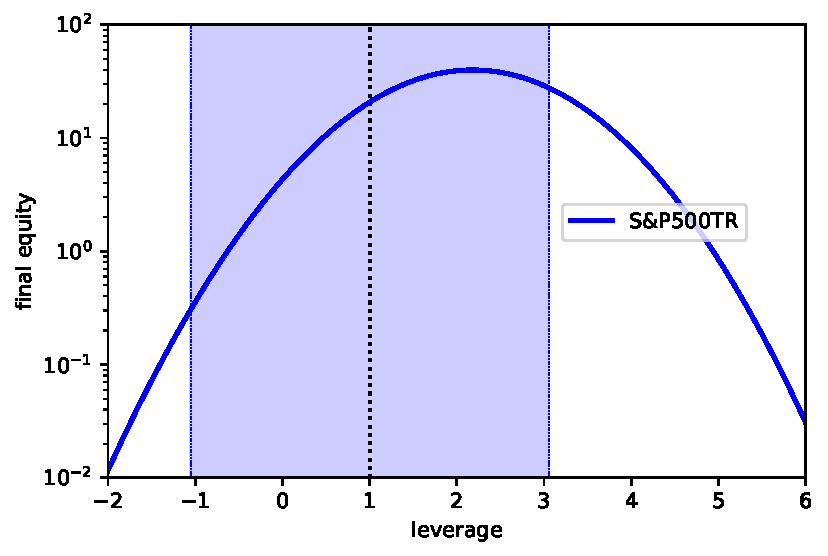
\includegraphics[width=\textwidth]{./all_final_equity_2.pdf}}
\end{picture}
\caption{\flabel{STR_final_all}}
\end{figure}

%
%\begin{figure}
%\centering
%\begin{picture}(200,300)(0,0)
%%  \put(0,0){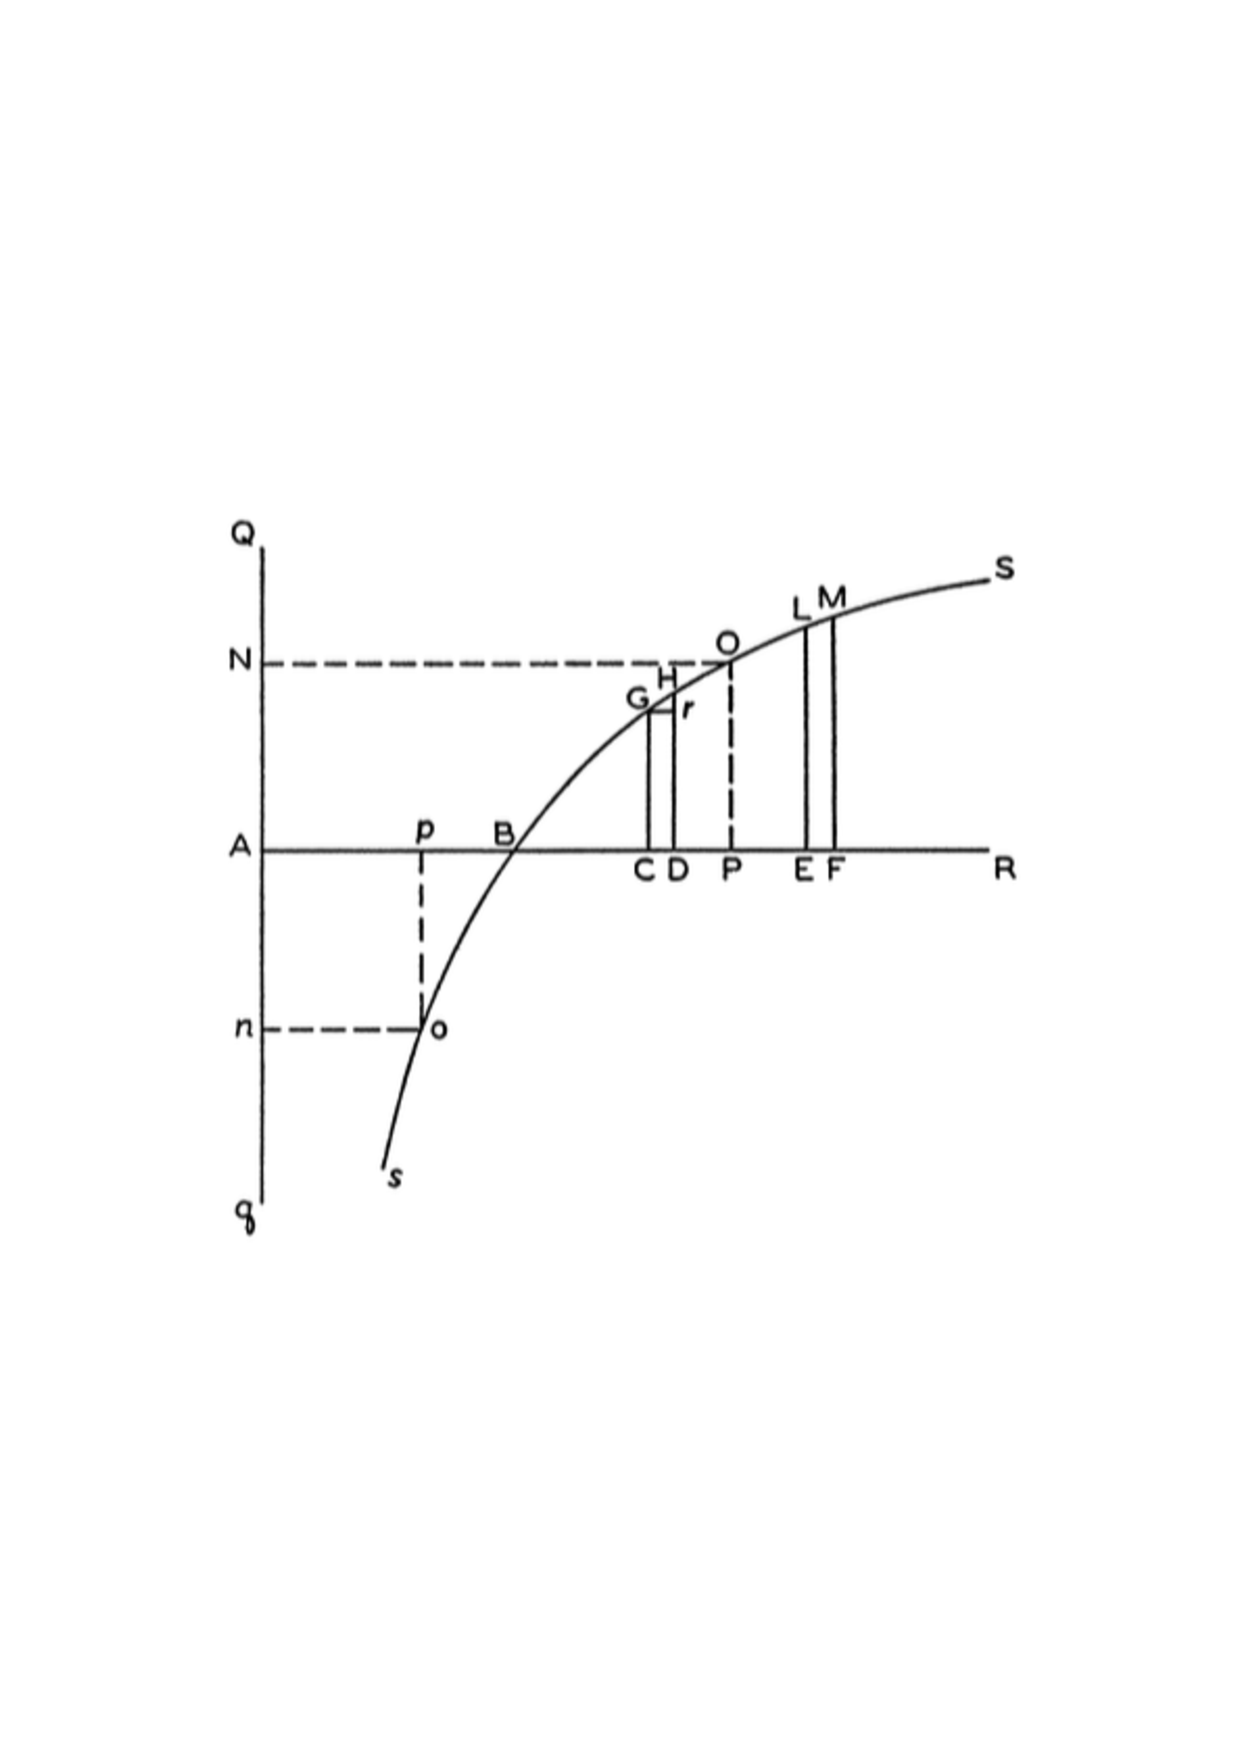
\includegraphics[width=.5*\textwidth]{./Untitled.pdf}}
%  \put(0,0){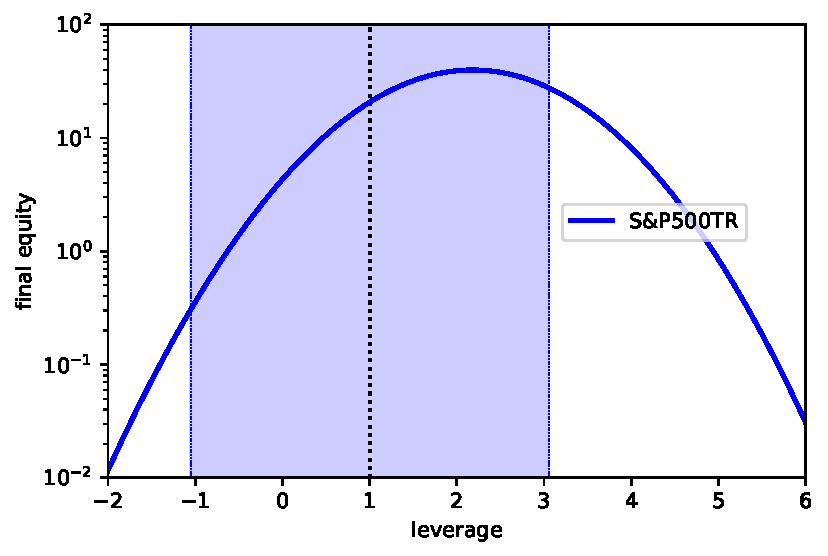
\includegraphics[width=\textwidth]{./all_final_equity_2.pdf}}
%\end{picture}
%\caption{}
%\flabel{key}
%\end{figure}


\section{Discussion}
It is impossible to reconcile Bernoulli's EUT with modern EUT. 
We are, however, free to speculate about the reasons for Bernoulli's inelegant theory. We may conclude that Bernoulli developed a different expected utility theory on purpose, and that, over the centuries, we diverged from his original vision. This argument is supported because Bernouilli is consisted in his use of \eref{ub} throughout his paper. 

Alternatively, we can interpret the difference between Bernoulli's EUT and modern EUT as an error that Bernoulli made when he wrote down the expectation value. In this view he contradicted himself, and his paper is inconsistent. This view is supported, in particular, by the following passage in the text that suggests Bernoulli actually wanted to compute $\ave{\Du}$ \cite[p.~24]{Bernoulli1738}: ``Meanwhile, let us use this as a fundamental rule: If the utility of each possible profit expectation is multiplied by the number of ways in which it can occur, and we then divide the sum of these products by the total number of possible cases, a mean utility will be obtained, and the profit which corresponds to this utility will equal the value of the risk in question.'' This suggests that Bernoulli wanted to compute $\ave{\Du}$, but the omission of an equation here leaves the statement open to interpretation: Did Bernoulli mean ``net profit'' when he wrote ``profit,'' or does he refer to a prize won?

I consider the second possibility more likely, and it seems Laplace agrees with me. Laplace presents the modern form of EUT that computes $\ave{\Du}$ as a criterion for gamble participation and ascribes it to Bernoulli, despite the fact that Bernoulli strictly put forward a different theory and did not compute this object. It must also be borne in mind how early in the development of probability theory, mathematics, and of course economics Bernoulli's study sits. Probability theory was in its infancy, and precisely the concepts Bernoulli stumbles over were still fluid an in the process of being developed. An example is the fact that a function of a random value $u(x)$ defines a new random variable (see \secref{Mathematical}) whose expectation value is not trivially related to the expectation value of $X$, meaning $\ave{u(x)}\neq u(\ave{x})$.

It is my impression that the inconsistency between Bernoulli's version of EUT and our modern form of EUT has caused a great deal of confusion. For instance, Karl Menger's famous result that utility functions must be bounded \cite{Menger1934} makes use of Bernoulli's original work and falls apart when one tries to base it on modern EUT \cite{Peters2011c,PetersGell-Mann2016}. According to XX this result is now ``routinely ignored'' yet it persists in the literature without having been thoroughly discarded. Similarly, discussions of prospect theory and cumulative prospect theory often confusingly claim that EUT misses a reference value. At this level of generality this statement is not true: EUT contains a reference value, namely present wealth. This may be related to the problem under investigation: if we insist that Bernoulli's and modern EUT are equivalent, we are forced to assume linear utility, and in that special case the reference value, $x$, cancels out from the computation of the decision criterion $\ave{\Du}$.
\bibliographystyle{plain}
\bibliography{bibliography}
\end{document}

